\section{Versuchsaufbau und Durchführung}
\label{sec:Durchführung}

Der Versuch ist \autoref{fig:aufbau} entsprechend aufgebaut.
\begin{figure}
    \centering
    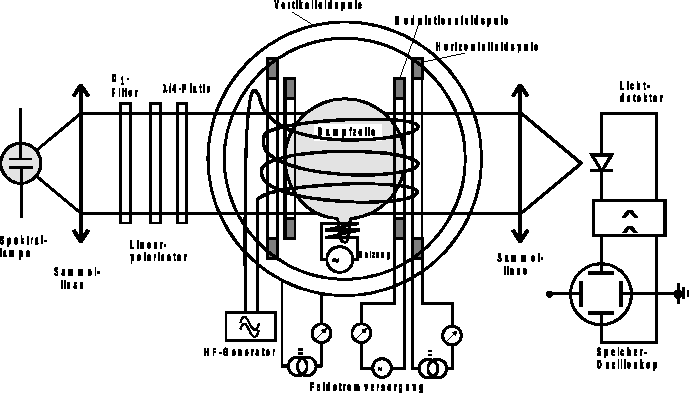
\includegraphics{figures/Aufbau.pdf}
    \caption{Schematische Darstellung des verwendeten Versuchaufbaus \cite{v21}.}
    \label{fig:aufbau}
\end{figure}

Eine Rubidium-Spektrallampe wird verwendet, um das in der Dampfzelle vorhandene Rubidium zu pumpen.
Da Rubidium bei Raumtemperatur fest ist, muss die Dampfzelle zunächst erhitzt werden, sodass das Rubidium in die Gasphase übergeht.
Das Licht, das von der Spektrallampe emittiert wird, muss, um zum optischen Pumpen genutzt werden zu können, zunächst geeignet polarisiert werden.
Dazu wird es durch den Polarisationsfilter zuerst linear und anschließend durch das $\lambda/4$-Plättchen zirkular polarisiert.
Hat das Spektrallicht die Dampfzelle durchdrungen, wird es mithilfe einer Sammellinse auf einen Photomultiplier fokussiert, der mit einem Oszilloskop verbunden ist.\\

Um die Dampfzelle selbst sind einige Spulenpaare angebracht.
Zwei der Helmholtzspulenpaare dienen der Kompensation der horizontalen und vertikalen Komponente des bei der Messung störenden Erdmagnetfelds.
Die dritte, sogenannte Sweep-Spule ist in der Lage, das Magnetfeld in einer bestimmten Zeit zwischen einer definierten Start- und Endmagnetfeldstärke zu variieren.
Die Sweep-Spule verfügt über $N = 11$ Windungen mit einem mittleren Radius von $R = \SI{16.39}{\centi\meter}$, das Vertikalspulenpaar besitzt die Parameter $N = 20$ und $R = \SI{11.735}{\centi\meter}$ und
das Horizontalspulenpaar $N = 154$ und $R = \SI{15.79}{\centi\meter}$.

\subsection{Justierung und Durchführung}

Vor Beginn der eigentlichen Messreihe muss der Aufbau justiert werden.
Die Sammellinsen, der Polarisationsfilter und das $\lambda/4$-Plättchen werden dazu so eingebaut, dass die am Oszilloskop beobachtete Intensität maximal wird.
Nun wird durch die Variation des Vertikalfeldes die vertikale Komponente des Erdmagnetfelds kompensiert. 
Der Aufbau wird zusätzlich nach Norden ausgerichtet, um die Horizontalkomponente des Erdmagnetfelds zu kompensieren.
Am Oszilloskop sollte dabei ein Peak erkennbar sein, der je nach Orientierung und Vertikalfeld schmaler oder breiter wird.
Dieser Peak soll möglichst schmal werden.

Ist der Aufbau justiert, kann mit der Messung begonnen werden. 
Dazu wird die Frequenz am Frequenzgenerator in $\SI{100}{\kilo\hertz}$-Schriiten von $\SI{100}{\kilo\hertz}$ auf $\SI{1}{\mega\hertz}$ erhöht.
Über das Verändern des Sweepspulenbereichs können so die Positionen der Peaks am Oszilloskop genau bestimmt werden.